\documentclass[11pt,a4paper]{article}
\pdfoutput=1
%vons grund
\usepackage[utf8]{inputenc}
\usepackage[T1]{fontenc}
\usepackage[german, english, swedish]{babel} %OBS! Se till att vi får rätt språk.
\usepackage{amsmath}
\usepackage{lmodern}
\usepackage{units}
\usepackage{icomma}
\usepackage{color}
\usepackage{graphicx}
\graphicspath{ {bilder/} }
\usepackage{bbm}
\newcommand{\N}{\ensuremath{\mathbbm{N}}}
\newcommand{\Z}{\ensuremath{\mathbbm{Z}}}
\newcommand{\Q}{\ensuremath{\mathbbm{Q}}}
\newcommand{\R}{\ensuremath{\mathbbm{R}}}
\newcommand{\C}{\ensuremath{\mathbbm{C}}}
\newcommand{\rd}{\ensuremath{\mathrm{d}}}
\newcommand{\id}{\ensuremath{\,\rd}}
\usepackage{hyperref}


%%%%%%%%%%%%%%%%%%%%%%%Egna tillägg%%%%%%%%%%%%%%%%%%%%%%%
%%För att få referenser 'på svenska'
%\usepackage[]{babelbib}
%\selectbiblanguage{english}
%\renewcommand\btxauthorcolon{:}
%%För att figurtext i underfigurer
\usepackage{subfigure} 
%%För att kunna inkludera andra PDF-dokument
\usepackage{pdfpages}
%%För att kunna ha roterade bilder
\usepackage{rotating}
%%För att kunna byta uppräkningsvisare t.ex. [label=\alph*)]
\usepackage{enumitem}
%%För att kunna lägga till 'bilagor' utan sidnumrering.
\usepackage{tocstyle}
\usetocstyle{standard}%För att få en vanlig TOC
                %no page numbers for part
\settocstylefeature[-1]{pagenumberbox}{\csname @gobble\endcsname}
\usepackage[nottoc]{tocbibind} %Puts an 'Reference' entry in the ToC.
%%För att kunna använda bra och ket och mycket annat smått och gott
\usepackage{physics} %\bra{}\ket{} eller \expval{H}{\psi}
%%För att kunna rita snygga matriser
\usepackage{mathtools} %\begin{pmatrix*}[r] ... \end
%%För att kunna kommentera ut större stycken
%%Drar in tabell och figurtexter
\usepackage[margin=10 pt]{caption}
\usepackage{comment} %\begin{comment}
%%För att lägga in 'att göra'-noteringar i texten
\usepackage[disable]{todonotes} %\todo{...}, \todolist
%\renewcommand{\todo}{\todo {}}


%%För att inkludera MATLABkod. 
%%OBS: mcode är ett separat paket och man måste ha mcode.sty i samma
%%katalog som dokumentet.
%\usepackage[framed,numbered,autolinebreaks,useliterate]{mcode}
%\usepackage{listings} 
%\lstloadlanguages{matlab} 
%\lstset{language=matlab} 
%\lstset{literate= {å}{{\r{a}}}1 {ä}{{\"a}}1 {ö}{{\"o}}1 {Å}{{\r{A}}}1
%  {Ä}{{\"A}}1 {Ö}{{\"O}}1}%För att få svenska bokstäver från MATLAB.


%%%%%%%%%%%%%%%%%%%%%%%Formatering%%%%%%%%%%%%%%%%%%%%%%%%
%%Partiell derivata
\newcommand{\pd}{\ensuremath{\partial}}
%%Följer ISO-8601 oberoende av språk.
\usepackage[iso, swedish]{isodate}
%%Göra grader Celcius
\newcommand{\degC}{\ifmmode \,^\circ\mathrm{C} \else $\,^\circ\mathrm{C}$ \fi}
%%Figurreferenser
\newcommand{\figref}{\figurename~\ref} 
%%Tabellreferenser
\newcommand{\tabref}{\tablename~\ref} %Stor bokstav i början

%%Det ska vara ett rakt µ i prefixet
\usepackage{upgreek}
\newcommand{\micro}{\upmu}
%%Ohm enhetskommando
\newcommand{\ohm}{\ifmmode \Upomega \else $\Upomega$ \fi}

%%'e' och 'i' ska vara upprätt
\newcommand{\e}{\mathrm{e}}
\newcommand{\ii}{\mathrm{i}}


%%För att själv bestämma marginalerna. 
\usepackage[
%            top    = 3cm,
%            bottom = 3cm,
%            left   = 3cm, right  = 3cm
]{geometry}


\begin{document}

\renewcommand{\thefootnote}{\fnsymbol{footnote}}

%kortkommandon för mailaddresserna
\newcommand{\andsunds}{andsunds@student.chalmers.se}
\newcommand{\rigon}{rigon@student.chalmers.se}



\pagenumbering{roman} %%Romersk sidnumrering i början
\begin{titlepage}
\newgeometry{top=3cm, bottom=2cm}

\newcommand{\HRule}{\rule{\linewidth}{0.5mm}} % Defines a new command for the horizontal lines, change thickness here

\center % Center everything on the page
 
%------------------------------------------------------------------------------------
%	HEADING SECTIONS
%------------------------------------------------------------------------------------

\textsc{\huge Chalmers tekniska högskola}\\[1.5cm] % Name of university/college
\textsc{\Large Rapport, Experimentell fysik 2}\\[0.2cm] % Major heading such as course name
\textsc{\large Termodynamik -- Uppgift 3 }\\[0.5cm] % Minor heading such as course title

%------------------------------------------------------------------------------------
%	TITLE SECTION
%------------------------------------------------------------------------------------

\HRule \\[0.4cm]
{ \LARGE \bfseries 
Studier av kvicksilveratomens atomära emissionsspektra samt absorptionsspektra av laserfärgämnena Rhodamin B och Kumarin 307
}\\[0.4cm] % Title of  document
\HRule \\[1.5cm]
 
%------------------------------------------------------------------------------------
%	AUTHOR SECTION
%------------------------------------------------------------------------------------

\begin{minipage}{0.4\textwidth}
\begin{flushleft} \large
\emph{Författare:}\\
Andréas Sundström\footnotemark{} \\
Rigon Demisai\footnotemark{} 
\end{flushleft}
\end{minipage}
~
\begin{minipage}{0.4\textwidth}
\begin{flushright} \large
\emph{Labassistent:} \\
Martin Wersäll
\end{flushright}
\end{minipage}\\[3cm]

\setcounter{footnote}{0}
\stepcounter{footnote}
  \footnotetext{\href{mailto:\andsunds}{\texttt{\andsunds}}}
\stepcounter{footnote}
  \footnotetext{\href{mailto:\rigon}{\texttt{\rigon}}}



%------------------------------------------------------------------------------------
%	DATE SECTION
%------------------------------------------------------------------------------------
% Följer ISO-standarden för tidsintervall:
% https://en.wikipedia.org/wiki/ISO_8601#Time_intervals
% "Double hyphen" också ok istället för '/'. -- i LaTeX är dock lite på gränsen
{ \large
\begin{tabular}{rc}
    Laboration utförd: & 2015-12-11/15 \\[0.1cm]
    Rapport inlämnad: & \today
\end{tabular}\\[1cm]
}

%------------------------------------------------------------------------------------
%	LOGO SECTION
%------------------------------------------------------------------------------------


\includegraphics[height=5cm]{logo.pdf} % Include a department/university logo
 
%------------------------------------------------------------------------------------

\vfill % Fill the rest of the page with whitespace

\end{titlepage}
\restoregeometry


\setcounter{page}{2}%detta är ANDRA (2) sidan

\renewcommand{\abstractname}{Sammandrag}
\begin{abstract}
Den här rapporten beskriver en spektroskopisk studie av
kvicksilveratomens atomära emissionsspektrum samt en studie av
laserfärgämnena rhodamin~B och kumarin~307 och deras
absorptionsspektra.
Ur emisionspektrumet från Hg har vissa av atomens energinivåer kartlagts,
baserat på kvanmekaniska regler och jämförelse med tidigare data på
Hg.  Kvicksilvrets emissionsspektra
är taget i intervallet 350--1100\,nm, där detekterades totalt 23
emissionstoppar, varefter 13 övergångar kunde identifieras.
Absorptionsspektrumen för rhodamin~B och kumarin~307 visar breda
absorptionsband vilket är kännetecknande för flourescerande ämnen som
består av stora organiska molekyler. 
Mätningarna har utförts med en Spex~270M spektrometer och
datainsamlingen har gjorts i LabView.
\end{abstract}

\renewcommand{\abstractname}{Abstract}
\begin{abstract}
This report describes a spectroscopic study of the atomic emision
spectrum of mercury, and also a study of the laser dyes Rhodamine~D
and Coumarin~307 and their absorption spectrum.
Som of the energylevels of Hg have been idetified from the emission
spectrum, based on quantum mecanichal rules and comparison with erlier
data on Hg. The emission spectrum of mercury was taken in the interval
of 350--1100\,nm, there a total of 23 emission lines were detected,
from which 13 different atomic transitions could be identified. 
The absorption spectrum of Rhodamin~B and Coumarin~307  show wide
absorption bands which are characteristic of big organic molecules.
THe measurements were made with a Spex~270M spectrometer and the data
collection was done through LabVIEW.
\end{abstract}

\clearpage
\renewcommand{\contentsname}{Innehållsförteckning}
\tableofcontents

\clearpage
\pagenumbering{arabic}
\setcounter{page}{1}

\renewcommand{\thefootnote}{\arabic{footnote}}
\setcounter{footnote}{0}





\section{Inledning}
Spektroskopi har varit, och är fortfarnde, ett kraftfullt verktyg för
exempelvis kemister och astronomer för att avgöra vad för grundämnen
och molekyler som undersöks. Tack vare att alla grundämnen har sina
egna emissions- och absorptionsspektra har man utan att direkt
tillgång till en substans kunnat avgöra dess innehåll genom dess
spektrum. 

Dessa spektra består vanligen av distinkta linjer. Och det beror på
att elektronerna bara kan ha vissa diskreta energinivåer i atomen. Så
är i alla fall fallet med \emph{atom}spektran. Men om större molekyler
undersöks så finns ofta många tätt liggande nivåer så att
spektrallinjerna blir ''utsmetade''. Detta är fallet med
t.ex. laserfärgämen -- ämnen som absorberat en kortare ljusvåglängd
och sedan via olika mellansteg emitterar ljus med en längre våglängd.

Bestämming av vilka ämnen som finns i ett prov må vara bland de
vanligaste tillämpningarna av spektroskopi. Men den här rapportens
syfte är att dels bestämma ett energinivådiagram från ett
atomspektrum, dels observera och förklara absorptionsspektrat från två
laserfärgämnen.  Denna rapport kommer specifikt studera
emissionspektrat för kvicksilver\footnotemark{} och
absorptionsspektrumen från två laserfärgämne och utifrån det
konstruera motsvarande energinivådiagram. 
\footnotetext{Anmärkning: Det var egentligen sagt att vi skulle
  undersöka Kadmium, men kadmiumlampan (eller aggregatet till den
  typen av spektrallampor) gick sönder när mätningarna skulle
  starta. På grund av att laborationen utfördes över en helg gick det
  inte att ersätta spektrallampan, så en annan lampa (med ett annat
  aggregat) fick användas istället. }


\subsection{Bakgrund}
Elektroner är bundna till atomkärnan i väldefinierade kvanttillstånd
kallade atomorbitaler. Varje sådant tillstånd har en väldefinierad
energi. Elektroner kan röra sig mellan energinivåerna genom att
absorbera eller emittera en foton med energi som matchar 
energiskillnaden mellan atomens orbitaler. 

En elektron kan ''hoppa'' till ett högre energitillstånd genom att absorbera en foton
som motsvarar den energi som krävs för nå en högre energinivå. Man
säger då att elektronen exciteras genom att \emph{absorbera} en
foton. Vid övergång från ett högre till lägre energitillstånd
\emph{emitteras} istället en foton med den frekvens som svarar mot
energiskillnaden mellan energinivåerna. 
 
Varje grundämne karakteriseras av en unik sammansättning av
elektroner och orbitaler som är bundna till kärnan i unika
konfigurationer. Detta leder till att energinivåerna är unika för
varje grundämne varför spektroskopi är ett kraftfullt verktyg för
ämnesbestämming. 
 
Genom att studera vilka ljusvåglängder som emitteras från ett prov
kan alltså de olika energiskillnadera bestämmas med hjälp av  
\[\Delta E = h\nu=\frac{hc}{\lambda}.\]
På så sätt kan alla energinivåer (med $\Delta E$ i de detekterbara
våglängderna) bestämmas relativt varandra. Att bestämma de absoluta
energierna på varje nivå är svårare. Man skulle kunna tänka sig
utnyttja att de högsta energinivåerna ligger mycket tätt och därmed
kommer att bidra till ett något diffust band i spektrat. Det finns då
ett sådant band för varje ''lägre'' eneginivå och på så sätt skulle
dessa energinivåer kunna bestämmas absolut. Dock är det mycket svårt
att avgöra vilket band som hör till vilken lägre energinivå annan än
för väteatomen. 
 
Ett annat hjälpmedel i bestämmandet av energinivåerna är de så
kallade urvalreglerna 
\begin{equation*}
\begin{aligned}
\Delta l &= \pm 1\\
\Delta m &= 0, \pm 1.
\end{aligned}
\end{equation*}
Dessa bestämmer hur det azimutala kvanttalet $l$ och det magnetiska
kvanttalet $m$ kan ändras. För den här laborationen kommer
framförallt urvalsregeln för $l$-kvanttalat att vara av intresse. 


\section{Metod}
%

Spektroskopi är en ganska rättfram mätmetod. Man har ett prov som man
kan erhålla ljus ifrån. Ljuset leds sedan in i en monokromator och som
plockar ut en specifik våglängd. Efter monokromatorn mäts
ljusintensiteten för alla våglängder man är intresserade utav. På så
sätt fås spektrumet fram.

Dessa mätningar kommer i stort sett går ut på att sakta arbeta sig
igenom spektrometerns mätområde och registrera ljusintensiteten. Detta
görs lämpligast digitalt med t.ex. ett program i LabView som styr
spektrometern och lagrar intensitetsdata. 


\subsection{Energinivåbestämmning}
Spektrallinjerna ger oss information om energiskillnaden mellan två
energinivåer, men inte om vilka nivåer det är talan om. Vi får på egen
hand försöka bestämma de relativa energinivåerna genom att para ihop
olika spektrallinjer (energiskillnader) och sedan förlita oss på bland
annat urvalreglerna och sålla bort förbjudna kombinationer av
övergångar.

\subsection{Absorption i lösningar}
För att studera absorptionsspektrumet för ett prov är grundtanken
ganska enkel: man lyser en lampa med känt spektrum på provet och ser
\href{https://xkcd.com/1517/}{hur det transmitterade ljuset skiljer
  sig från ursprungsspektrumet}. I verkligheten behöver man vara lite
mer vaksam. 

Till att börja med så har vi det ''kända spektrumet''. Det man får
göra där är att göra en torrkörning\footnotemark av sin mätning för
att få hur det opåverkade spektrumet ser ut. Detta bör göras även om
man redan känner till spektrumet för att veta hur den opåverkade
intensiteten är och hur t.ex. provbehållare påverkar ljuset. 
\footnotetext{''Torrkörningen'' innebär inte nödvändigt vis att man
  gör en helt \emph{torr} mätning. Optimalt borde torrkörningen göras
  med enbart lösningsmedlet för att få bakgrundsreferensen. }

Sedan kan man köra en mätning med provet där man lyser lampan rakt
igenom provet och undersöker ljuset som kommer ut på andra sidan. Här
kan man dock behöva passa sig för ifall ens prov uppvisar fluorescens
och därmed kommer att resultera i en annan ''ljusbakgrund'' för
mätningen av absorption\cite{flour_spec}. Detta skulle man kunna
kontrollera genom att göra en spektralmäning från sidan för att se vad
ämnet självt emitterar för ljus -- denna mätning bör också ha
föregåtts av en torrkörning för att kalibrera bakgrunden. 




\section{Resultat}
Resultaten från en spektroskopisk mätning 



\newgeometry{top=3cm}%, bottom=3cm}
\begin{sidewaysfigure}\centering
\centerline{ %centrerar även större bilder
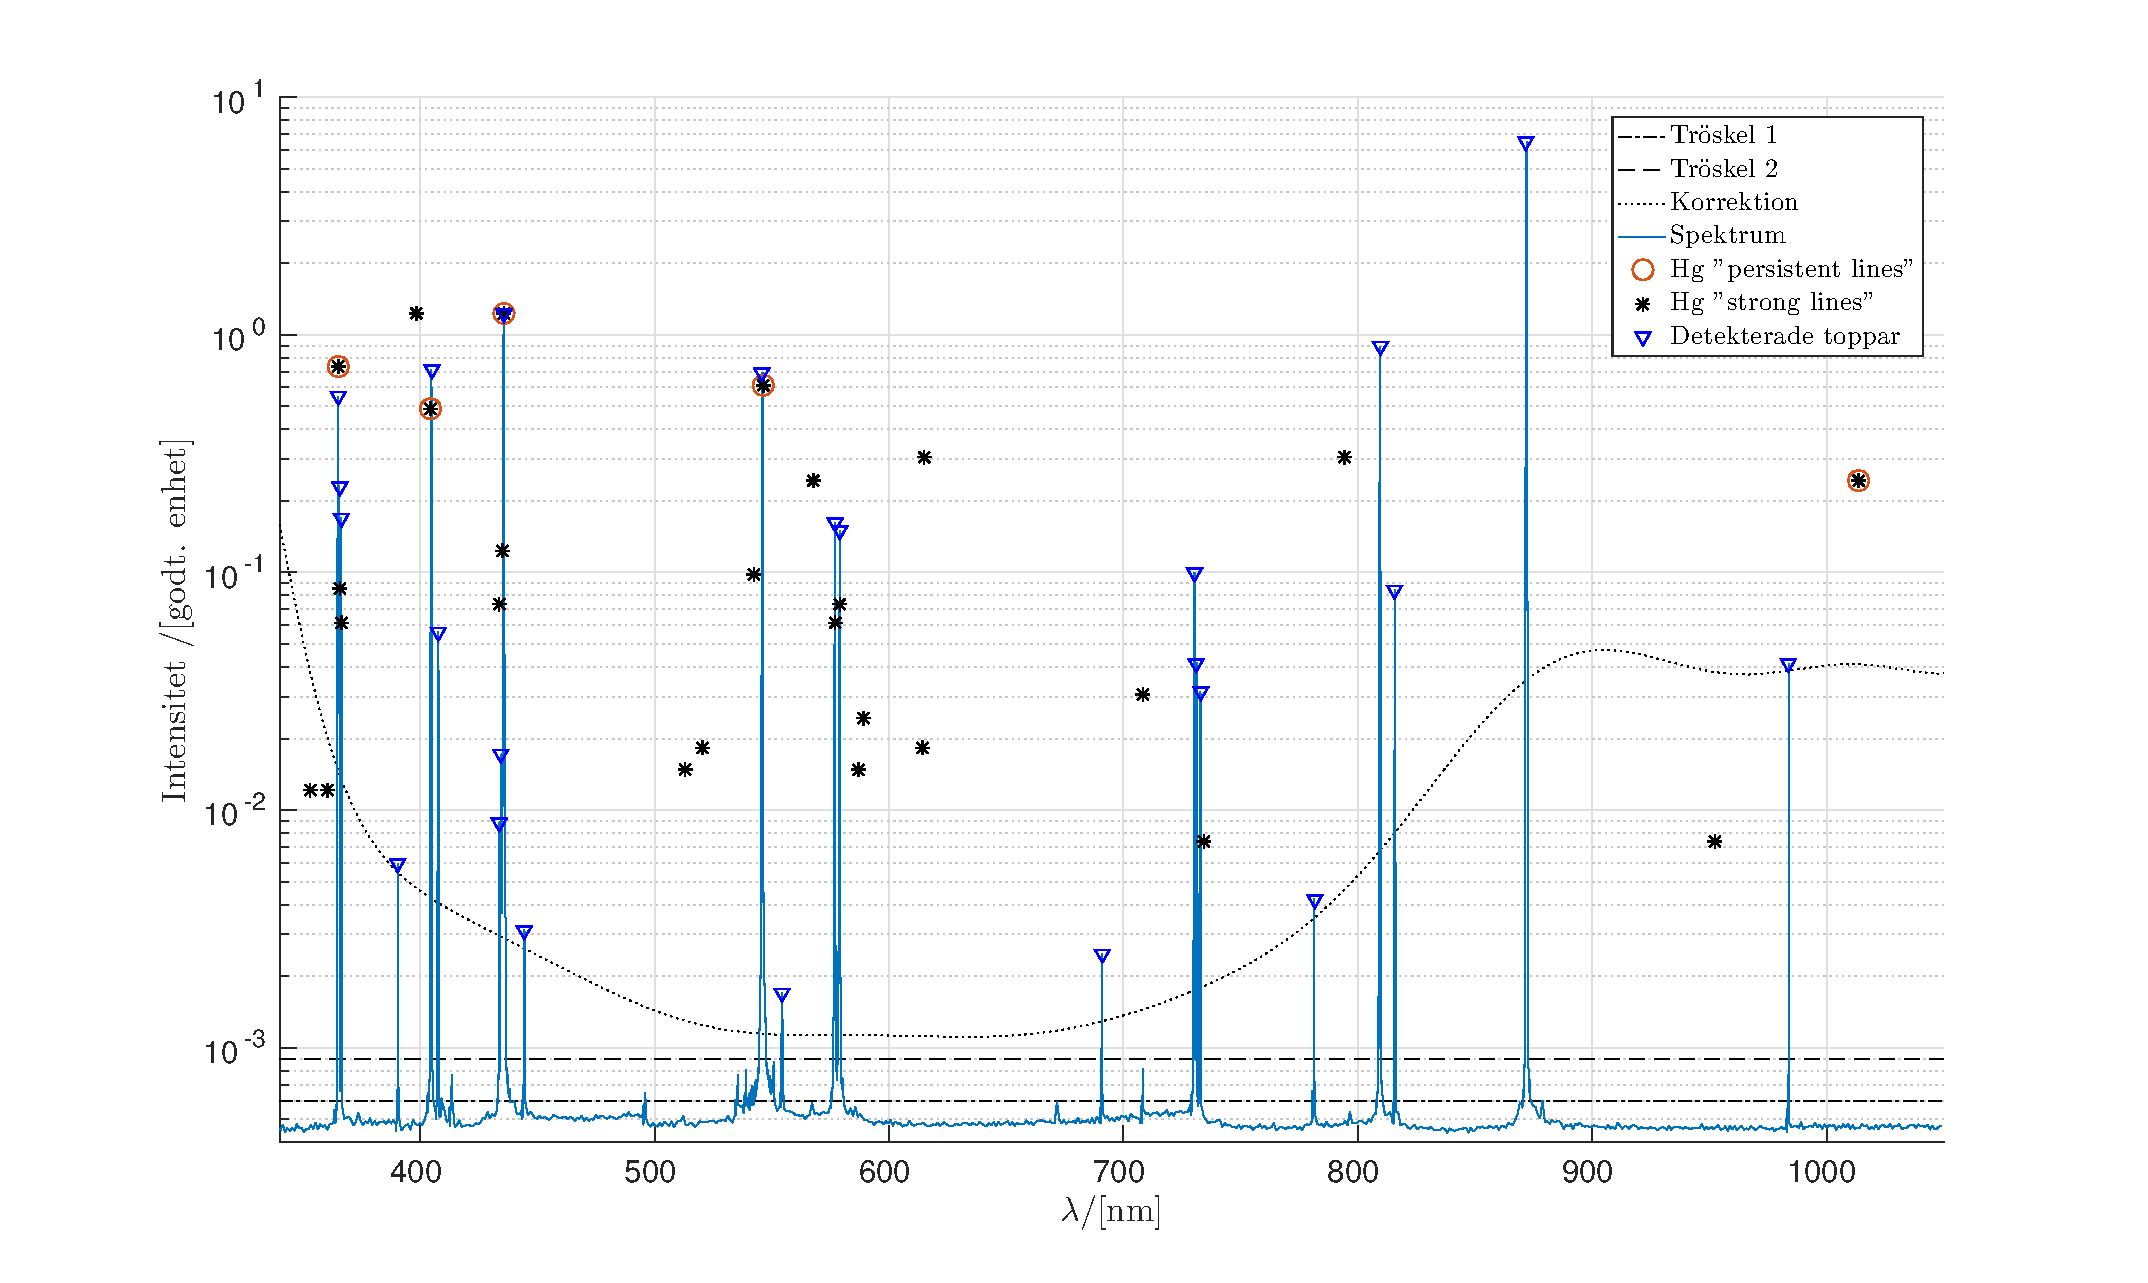
\includegraphics[width=1.2\textwidth]{Hg_spektrum.pdf}
}
\caption{Spektrum uppmätt från kvicksilverlampa tillsammans med
  utmarkerade spektraltoppar enligt NIST\cite{NIST}. De två olika
  typerna av tabellerade data från NIST kallas ''persistent''
  respektive ''strong lines''; skillnaden mellan dessa två tabeller är
  att ''persistent lines'' är de spektrallinjer som syns tydligast
  då det även förekommer orenheter i provet som kan blockera vissa
  övergångar, medan ''strong lines'' är alla starka spektrallinjer som
  förekommer hos ett rent prov.
  Av de två trösklarna som är utritade, styr den första när en en topp
  ska anses stor nog för att det ska vara intressant att minska
  steglängden i våglängd, och den andra tröskeln styr när korrektionen
  ska användas. Korrektionen används bara för de toppar som når över
  den andra tröskeln för att inte den bredare basen på en topp ska
  orsaka att hela toppen ser allt för bred ut. Notera att intensiteten
  är ritad med log-skala, vilket gör att korrektionsfaktorn effektivt
  adderas till toppens höjd varför korrektionen är utritad relativt
  tröskelvärdet och alltså inte motsvarande värdet som ges på
  intensitetsaxeln. 
}
\label{fig:Hg_spektrum} 
\end{sidewaysfigure}
\restoregeometry

\begin{figure}\centering
\centerline{ %centrerar även större bilder
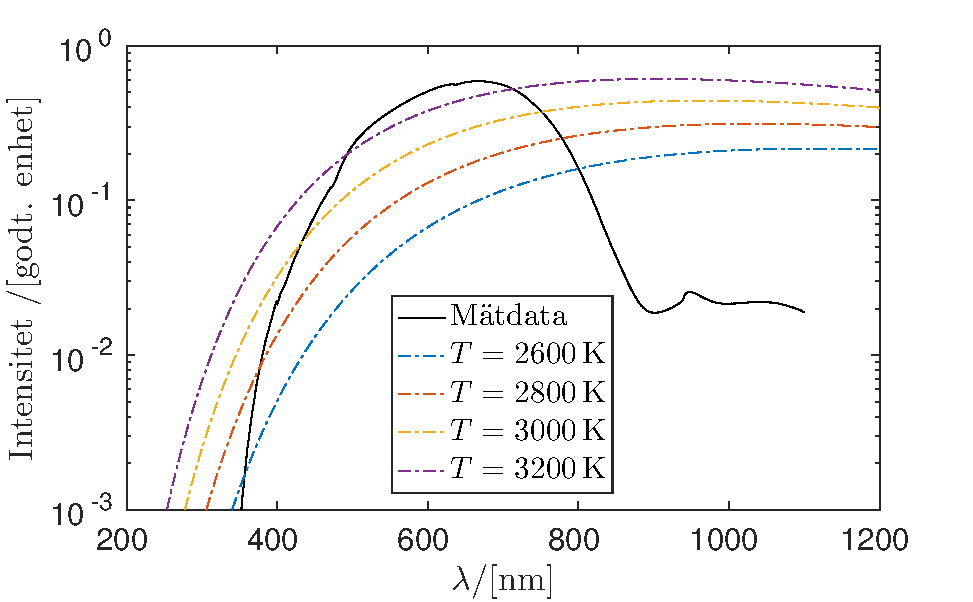
\includegraphics[width=.9\textwidth]{svartkropp.pdf}
}
\caption{Uppmätt spektrum (heldraget) med spektrometern från en
  glödlampa, jämfört med vad Plancks strålningslag ger (normerade
  kurvor). Härifrån syns tydligt att spektrometern har ett ganska
  snävt känslighetsområde där man helst inte bör gå mycket högre än
  till ca 800\,nm våglängd.}
\label{fig:svartkropp}
\end{figure}

\begin{figure}\centering
\centerline{ %centrerar även större bilder
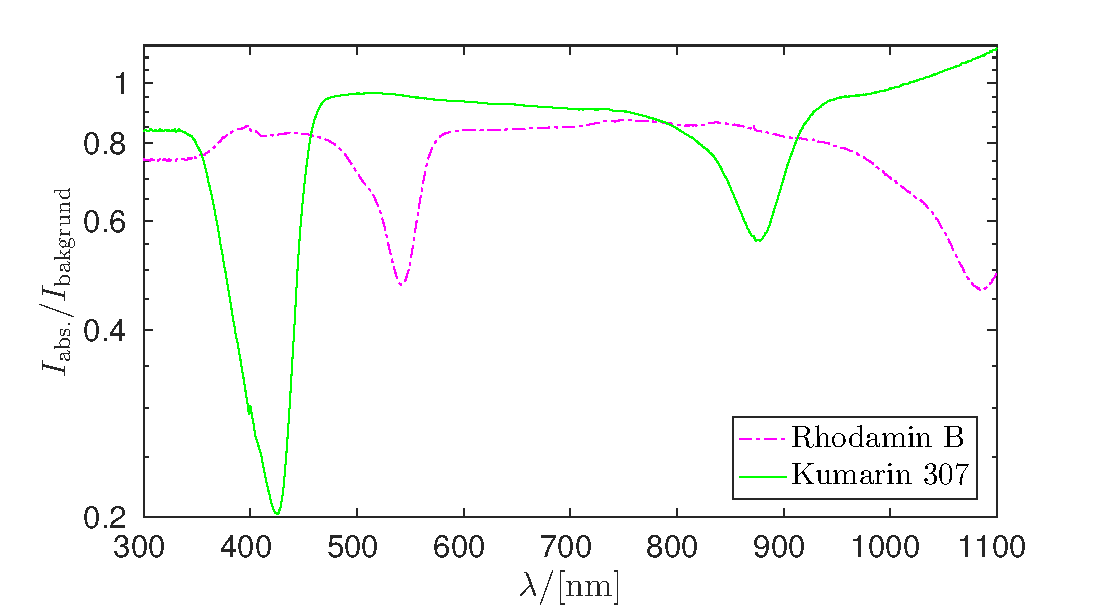
\includegraphics[width=1\textwidth]{absorption.pdf}
}
\caption{Absoprtionsspektrum från Rhodamin B och Kumarin
  307. Absorptionsspektrumen är framtagna som kvoten mellan
  intensiteten som lyste igenom provet mot intensiteten från samma
  ljuskälla utan något prov. Spektrat frånglödlampan som användes som
  ljuskälla visas i \figref{fig:svartkropp}. 
}
\label{fig:absorption} 
\end{figure}



\section{Diskussion}
I uppgiften med att identifiera energinivåerna i en atom nämndes att
det är lätt att identifiera de olika energinivåernas inbördes avstånd,
men att det kan bli svårt att bestämma de absoluta energierna. 

Det är förvisso sant att det förmodligen inte kommer gå att bestämma
de absoluta energierna, men även alla inbördes energiskillnader kan
bli vanskliga att ta fram. Från spektroskopin kommer vi att få ut ett
antal våglängder som svarar mot en viss energi\-skillnad mellan två
nivåer. Här måste man nu vara vaksam. Det är ju oftast inte så att
alla övergångar sker från en viss nivå till den lägsta möjliga nivån;
vissa övergångar kan ju ske mellan två exciterade tillstånd. Man får
alltså se om man kan passa ihop flera våglängder svarande mot
övergångar dels från en exciterad nivå till grundnivån, dels från en
exciterad nivå till en mellannivå och sen till grundnivån. Detta kan
bli lite pilligt men inte omöjligt att göra. I övrigt upplevs
bestämmadet av energinivåerna inte så svårt. 

För undersökningen av absorption i lösning har vi på förhand inte så
mycket att utgå från. Vi har åtminstone att lösningsmedlet lär påverka
energinivåerna i molekylen/jonen. Tidigare resultat för olika
organiska färgämnen påvisar ett frekvensskift av absorptionstoppen
beroende på hur polärt lösninsmedlet är \cite{Mannekutla2008}, men
olika lösningmedel kan även starkt påverka absorptionens intensitet
\cite{Homocianu2011}.
I övrigt finns det annat som kan påverka absorptionsspektrat som
exempelvis jonladdning om man undersöker metalljoner i lösning. 

Andra förväntade resultat för mätningen av laserfärgämnena är som
nämnts tidigare att de kommer att sakna distinkta toppar och att de
flourescerar med längre våglängder än det absorberar. 

\subsection{Hg-spektrum}
%Fattas toppar

\subsubsection{För många toppar}

\subsection{Absorptionsspektrum}
%Varför breda dalar och inte skarpa spikar?

\subsection{Upptagningen av spektrumen}
%Enpunktskalibrering
%Känslighetsområde








%För att lägga in en referens så ska den skrivas in enligt mönstret i filen referenser.bib
%Använd \cite{} som vanligt för att använda referensen i texten.
%Här är en bra länk om hur man ska göra:
%https://en.wikibooks.org/wiki/LaTeX/Bibliography_Management#biblatex

\newpage
\iflanguage{swedish}{\renewcommand{\refname}{Källförteckning}}{}
\bibliographystyle{ieeetr}
\bibliography{referenser}


%Detta ser till att bilagorna kommer in snyggt i rapporten/förstudien
\clearpage
\appendix
\setcounter{page}{1}
\renewcommand*{\thepage}{A\arabic{page}}
\phantomsection{}
\iflanguage{swedish}{\renewcommand{\appendixname}{Bilagor}}{}
\addcontentsline{toc}{part}{\appendixname}
\iflanguage{swedish}{\renewcommand{\appendixname}{Bilaga}}{}

\section{Korrektion}

\begin{figure}\centering
\centerline{ %centrerar även större bilder
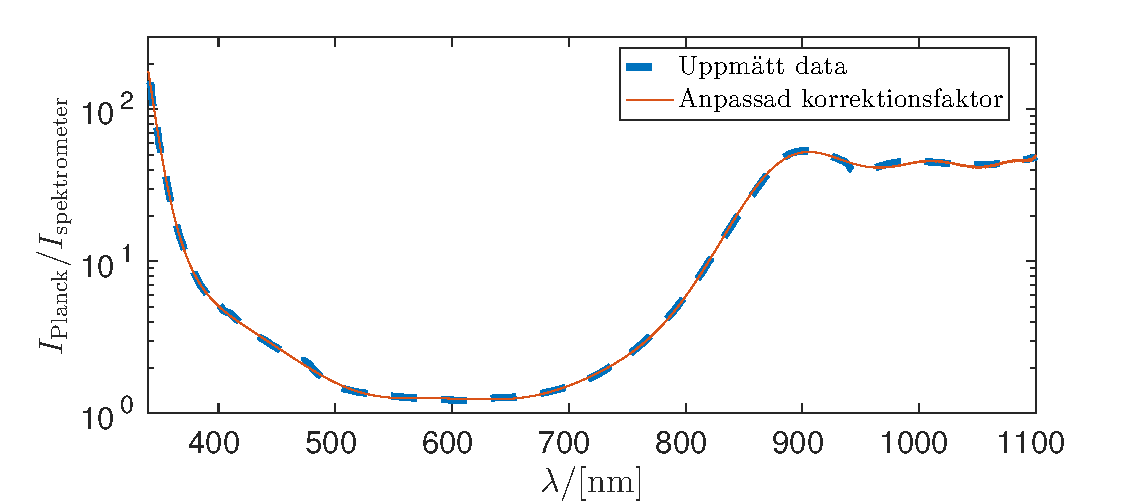
\includegraphics[width=.9\textwidth]{korrektionsfaktor.pdf}
}
\caption{\label{fig:korrektionsfaktor} }
\end{figure}

\begin{figure}\centering
\centerline{ %centrerar även större bilder
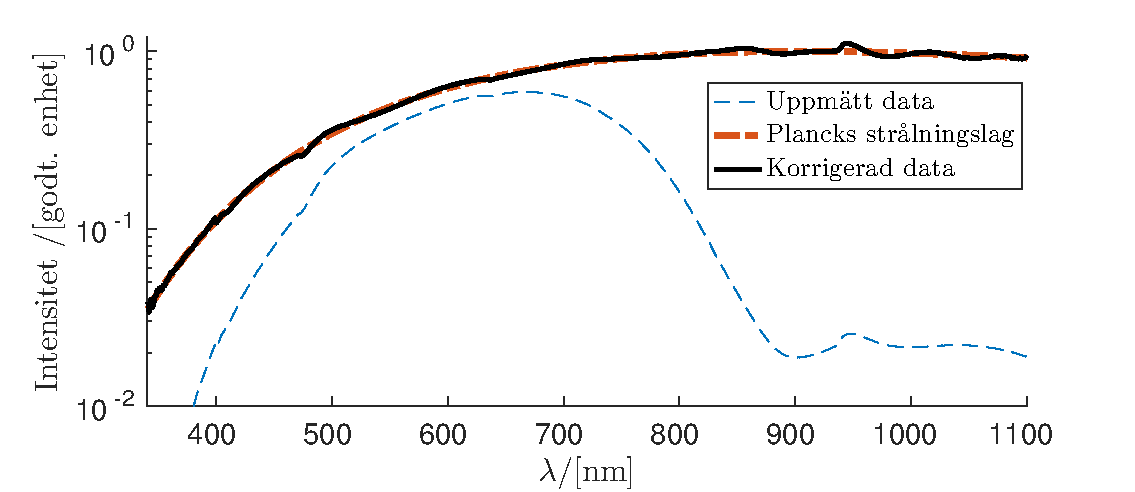
\includegraphics[width=.9\textwidth]{anpassad_svartkropp.pdf}
}
\caption{\label{fig:anpassad_svartkropp} }
\end{figure}


\end{document}


%% På svenska ska citattecknet vara samma i både början och slut.
%% Använd två apostrofer (två enkelfjongar): ''.

%%För att referera till till tidigare fotnot:
%    \footnotemark[\value{footnote}]

%% Figurer inkluderade som pdf-filer
%\begin{figure}\centering
%\centerline{ %centrerar även större bilder
%\includegraphics[width=1\textwidth]{filnamn.pdf}
%}
%\caption{\label{figuren} Perioden $T$ som funktion av pendellängden.}
%\end{figure}

%% Figurer inkluderade med xfigs "Combined PDF/LaTeX"
%\begin{figure}\centering
%\input{filnamn.pdf_t}
%\caption{\label{finafiguren} Perioden $T$ som funktion av
%  pendellängden.}
%\end{figure}

%http://www.ict.kth.se/courses/IO2651/docs/ElectroOptics_paper.pdf

%Förstärkare:
%http://www.thinksrs.com/products/SR445A.htm